\chapter{Lecture 2: SVD}
In this lecture we look at singular value decomposition (SVD) and the relation to PCA. To get a more intuitive sense of the material here, I suggest the following: http://www.ams.org/publicoutreach/feature-column/fcarc-svd.
\section{Small recap of linear algebra}
This section is very incomplete, it is recommended to find a better source for basic linear algebra.
\subsection{Diagonalization}
When can you diagonalize a matrix $A \in \Real^{n*n}$? A matrix can be diagonalized if and only if there exists a basis of $\Real^m$ consisting of eigenvectors of $A$. Then A can be diagonalized as follows:
\begin{equation}
\label{eq:diag}
P^{-1}AP = \begin{bmatrix}
			\lambda_1 & & \\
			&\ddots & \\
			&& \lambda_m\\
			\end{bmatrix}
\end{equation}
With the columns of $P$ consisting of the eigenvectors of $A$.
\paragraph{Example}
Take for instance following matrix $A$:
\begin{equation}
A = \begin{pmatrix}
0 & a \\
a & 0
\end{pmatrix}
\end{equation}
Finding it's eigenvectors means solving $Av = \lambda v$ for $\lambda$ and using it to find the eigenvectors. The equation $(A-\lambda\ID)v = 0$ has non trivial solutions if the determinant of it is zero (Cramer's rule):
\begin{equation}
\Det{A-\ID\lambda} = 0 
\end{equation}
This can easily seen to lead to the following characteristic polynomial:
\begin{equation}
\begin{split}
\lambda^2 - a^2 &= 0\\
\lambda &= \pm a
\end{split}
\end{equation}
Then using these eigenvalues we find the eigenvectors by solving $(A-\lambda\ID)v = 0$ we find that $v_1 = (\theta, \theta)$ for $\lambda_1 = a$ and $v_2=(\theta,-\theta)$ for $\lambda_2=-a$ with $\theta \in \Real$. We now see:
\begin{equation}
Av_1 = \hVec{a\theta\\a\theta} =av_1 = \lambda_1v_1 \text{ and } Av_2 = \hVec{-a\theta\\a\theta}=-av_2= \lambda_2v_2
\end{equation}
Applying $P^{-1}AP$ we obtain:
\begin{equation}
\begin{split}
\frac{1}{2a \theta }
\begin{pmatrix}
1 & 1\\
1 & -1\\ 
\end{pmatrix}
\begin{pmatrix}
0 & a\\
a & 0\\
\end{pmatrix}
a\theta
\begin{pmatrix}
1 & 1\\
1 & -1\\ 
\end{pmatrix} &=
\frac{1}{2}
\begin{pmatrix}
a & a\\
-a & a \\
\end{pmatrix}
\begin{pmatrix}
1 & 1\\
1 & -1\\ 
\end{pmatrix}\\
&= \begin{pmatrix}
a & 0\\
0 & -a\\
\end{pmatrix}\\
&= \begin{pmatrix}
\lambda_1 & 0 \\
0 & \lambda_2 \\
\end{pmatrix}
\end{split}
\end{equation}
So if a matrix is symmetric we can diagonalize it.
\subsection{Range and rank}
We look now at the range and rank of a matrix.
\begin{defn}
	The range of a matrix $A$ is defined as all the vectors the matrix $A$ can reach from it's domain:
	\begin{equation}
	\text{range}(A) = \{z|\exists x \in \text{Dom}(A) : z = Ax\}
	\end{equation}
	It is all possible linear combinations of the columns of $A$, it is also referred as the span of $A$.
\end{defn}
Another important concept we look at is the rank of matrix:
\begin{defn}
	The rank of matrix $A$ is defined as the dimension of range of $A$. 
	\begin{equation}
	\text{rank}(A) = \text{dim}(\text{range}(A))
	\end{equation}
\end{defn}
In the case of a diagonal matrix it is easily seen to be the amount of non-zero entries.
\begin{defn}
	The kernel of a matrix $A \in \Real^{m\times n}$ is the collection of points which map to the zero vector:
	\begin{equation}
	\text{Kernel}(A) = \{x|Ax=0\}
	\end{equation}
\end{defn}
\begin{thm}
	Rank-nullity therom:
	\begin{equation}
	\text{dim}(\text{kernel}(A)) + \text{dim}(\text{range}(A)) = n
	\end{equation}
\end{thm}
This theorem implies that if there are 
\section{Collaborative filtering}
This lecture will look a bit at collaborative filtering. Some practical applications for collaborative filtering are recommender systems e.g. used by Amazon, Netflix, Pandora, etc.
\paragraph{Example}
For example the Netflix database might consist of a huge matrix $X \in \Real^{n\times m}$ where $n$ is the amount of users and $m$ the movies available on netflix. The values in the matrix represent scores that users have given a particular movie. Of course this matrix will be extremely sparse. However if we want to recommend certain movies to certain users we could take the approach of "matrix completion" where we try to fill in missing values in the matrix.

\section{Matrix completion}
So how could we complete the matrix and fill in missing values according to the available data? One approach could consists of finding certain statistical relationships between certain entities and using this relation to infer missing values in the matrix. This approach to matrix completion is a statistical model.\\
Another approach could consist of finding a low rank composition. For this second approach we first look at a well known method of doing such a decomposition, namely the singular value decomposition or SVD.
\section{SVD}
The core concept of SVD is the following:
\begin{figure}[h!]
	\centering
	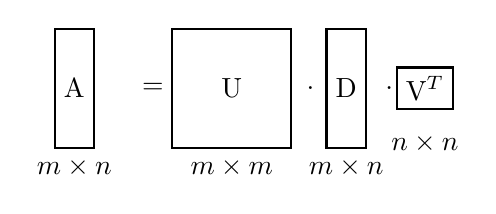
\begin{tikzpicture}
	\draw (0,0) node[shape=rectangle, draw = black, thick, minimum height=10ex](A){A};
	\draw node[below of = A]{$m\times n$};
	
	\draw node[right of = A](is){$=$};
	
	\draw node[right of = is, shape = rectangle, thick, minimum width = 10ex, minimum height=10ex, draw = black](U){U};
	\draw node[below of = U]{$m\times m$};
	
	\draw node[right of = U]{$.$};
	
	\draw node[right of = U, shape = rectangle, thick, minimum height=10ex, draw = black, xshift = 3ex](D){D};
	\draw node[below of = D]{$m\times n$};
	
	\draw node[right of = D,xshift = -3ex]{$.$};
	
	\draw node[right of = D, shape = rectangle, thick, draw = black](V){V$^T$};
	\draw node[below of = V, yshift = 2ex]{$n\times n$};
	\end{tikzpicture}
	\label{fig:core}
	\caption{Core concept of SVD visual.}
\end{figure}\\
Here the matrices $U$ and $V$ are orthogonal meaning that the columns and rows of the matrix are orthogonal i.e. $UU^T = U^TU = \ID_m$ and $D$ is diagonal depending on the dimensions $n$ and $m$:
\begin{figure}[h!]
	\centering
	\begin{tikzpicture}
	\draw (0,0) node[rectangle, minimum height = 10ex, minimum width = 10ex, draw=black](diag){$\begin{matrix}
		\sigma_1 & & \\
		& \ddots & \\
		&& \sigma_n\\
		\end{matrix} $};
	\draw node[below of = diag, shape = rectangle, draw = black, minimum width = 13.9ex, yshift = -1.1ex, minimum height = 4ex]{$0$};
	
	\draw (3,0) node[rectangle, minimum height = 10ex, minimum width = 10ex, draw=black](diag2){$\begin{matrix}
		\sigma_1 & & \\
		& \ddots & \\
		&& \sigma_m\\
		\end{matrix} $};
	\draw node[right of = diag2, shape = rectangle, draw = black, minimum height = 11.45ex, xshift = 2.5ex, minimum width = 4ex]{$0$};
	\end{tikzpicture}
	\label{fig:D}
	\caption{Different possibilities of the $D$ matrix.}
\end{figure}\\
On the diagonal are the singular values.\\

Taking a closer look at what exactly this means, we can first look at the term $UD$. From figure \ref{fig:D} we see that we only keep the $\min(m,n)$ first columns of the $D$ matrix:
\begin{equation}
\begin{pmatrix}
\vline &  & \vline& & \vline\\
v_1& \dots & v_n &\dots & v_m\\
\vline & & \vline& & \vline\\
\end{pmatrix}
\begin{pmatrix}
\sigma_1 & & \\
 & \ddots & \\
 &&\sigma_n\\
 0 & & \\
 & \ddots & \\
 & & 0\\
\end{pmatrix}
=
\begin{pmatrix}
\vline &  & \vline\\
v_1\sigma_1& \dots & v_n\sigma_n\\
\vline & & \vline\\
\end{pmatrix}
\end{equation}
So written out we indeed find the surviving vectors multiplied by their respective singular value $\sigma_i$. We then look at the next factor $V^T$:
\begin{equation}
\begin{pmatrix}
\vline &  & \vline\\
v_1\sigma_1& \dots & v_n\sigma_n\\
\vline & & \vline\\
\end{pmatrix}
\begin{pmatrix}
- & v_1 & -\\
& \vdots &\\
- & v_n & -\\
\end{pmatrix}
=
\begin{pmatrix}
a_{11} & & & & \\
& \ddots& & & \\
& & a_{ij} & & \\
& & & \ddots& \\
& & & & a_{mn}\\
\end{pmatrix}
\end{equation}
We can easily see $a_{ij}$ is interpreted as the sum over the vectors of the $i$'th component times the $j$'th component: $a_{ij}=\sum_{k=1}^{n} \sigma_ku_{ki}v_{kj}$. Taking the sum out we find:
\begin{equation}
\begin{split}
\sum_{k=1}^{n} \sigma_k
\begin{pmatrix}
u_{k1}v_{k1} & & & & \\
& \ddots& & & \\
& & u_{ki}v_{kj} & & \\
& & & \ddots& \\
& & & & u_{km}v_{kn}\\
\end{pmatrix}&=
\sum_{k=1}^{n} \sigma_k\hVec{u_{k1}\\\vdots\\u_{km}}\hVec{v_{k1} & \dots & v_{kn}}\\
&= \sum_{k=1}^{n}\sigma_k u_k v_n^T
\end{split}
\end{equation}
Note that the above derivations are identical for the case when $m < n$.
\subsection{Reduced SVD}
Note that a lot of computation in the decomposition is not usefull as it is multiplied with zeros. To see this note that in $DV^T$ and we assume that $n\geq m$:
\begin{equation}
\label{eq:reduced_svd}
DV^T = 
\begin{pmatrix}
\sigma_1 & & & 0 & & \\
& \ddots & & & \ddots & \\
&&\sigma_m & & & 0\\
\end{pmatrix}
\begin{pmatrix}
- & v_1 & -\\
& \vdots &\\
- & v_n & -\\
\end{pmatrix}=
\begin{pmatrix}
- & \sigma_1v_1 & -\\
& \vdots &\\
- & \sigma_m v_m & -\\
0 & &\\
&\ddots&\\
 & & 0\\
\end{pmatrix}
\end{equation}
From (\ref{eq:reduced_svd}) we can see that the zeros right from the diagonal matrix in:
\begin{equation}
D = 
\begin{pmatrix}
\underbrace{\tilde{D}}_{m\times m} & \underbrace{0}_{m\times (n-m)}\\
\end{pmatrix}
\end{equation}
Could be replaced by the $m\times m$ matrix $\tilde{D}$ and that in $V^T$ only the first $n$ rows need to be kept, so that:
\begin{equation}
\tilde{V}^T = \begin{pmatrix}
- & v_1 & -\\
& \vdots &\\
- & v_m & -\\
\end{pmatrix}
\end{equation} This results in the so called reduced svd:
\begin{equation}
A = \underbrace{U}_{m\times m} \underbrace{\tilde{D}}_{m \times m} \underbrace{\tilde{V}^T}_{m\times n}
\end{equation}
The reduced svd is computationally a lot better in the cases where your matrix is huge, most machine learning packages will offer a reduced svd alongside the full svd.

\subsection{Constructing an SVD}
So far only the general theory of SVD has been discussed, but is there an efficient way of actually constructing this decomposition as there was for the PCA? For SVD construction see algorithm \ref{alg:svd_construction}:\\

\begin{algorithm}
	\caption{Calculate $y = x^n$}
	\begin{algorithmic} 
		\STATE $U \leftarrow \emptyset$
		\STATE $V \leftarrow \emptyset$
		\STATE $B_1 \leftarrow A$
		\STATE $i \leftarrow 1$
	\end{algorithmic}
\end{algorithm}